\documentclass[pdf]{beamer}
\mode<presentation>{}

\usepackage[sans]{dsfont}
\usepackage{amsmath}

\newcommand{\op}[1]{\operatorname{#1}}
\newcommand{\bbf}[1]{\mathds{#1}}
\newcommand{\Z}{\bbf{Z}}

\title{Generic pro-$p$ Hecke algebras, the Hecke algebra of $\op{PGL}(2,\Z)$, and the cohomology of root data}
\subtitle{A thesis defense}
\author{Nicolas A. Schmidt}

\begin{document}

%% title frame
\begin{frame}
   \titlepage
\end{frame}

\begin{frame}{Das einfachste mathematische Objekt}
   \pause
   \begin{figure}
   \centering
      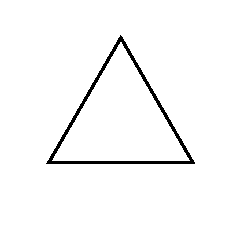
\includegraphics[width=0.5\textwidth]{graphics/triangle.eps}
   \end{figure}
\end{frame}

\end{document}
